% ACL Rolling Review long paper: 8 pages of content; Limitations, Ethical Considerations, references and appendices
% do not count. Official *ACL style files, unmodified (byte-identical to ssn-group-papaer/workbench/*/paper).
% Build both versions with ./build.sh: main.pdf (anonymous review copy) and main_arxiv.pdf (preprint, with authors).
% Figures: ../research/analysis/paper_figures.py; numbers: ../research/analysis/{paper_tables,residue_sets,item_slopes}.py.
\documentclass[11pt]{article}

\usepackage[review]{acl}
\usepackage{times}
\usepackage{latexsym}
\usepackage[T1]{fontenc}
\usepackage[utf8]{inputenc}
\usepackage{microtype}
\usepackage{inconsolata}
\usepackage{graphicx}
\usepackage{booktabs}
\usepackage{makecell}
\usepackage{amsmath,amssymb}
\usepackage{xcolor}
\usepackage[inline]{enumitem}
\usepackage{adjustbox}
\usepackage{tikz}
\usetikzlibrary{arrows.meta}
\definecolor{gpblue}{HTML}{2A78D6}
\definecolor{gporange}{HTML}{EB6834}

\newcommand{\ex}[1]{\textit{#1}}
\newcommand{\cond}[1]{\textsc{#1}}
\newcommand{\ci}[2]{{\scriptsize\,(#1, #2)}}
\makeatletter\newcommand{\rows}[1]{\@@input #1 }\makeatother

\title{Language Models Cannot Unread a Garden Path:\\ Abandoned Analyses Persist While Errors Drive Adaptation}

\author{Anonymous ACL submission}

\begin{document}
\maketitle

\begin{abstract}
When a reader meets \ex{While the man hunted the deer ran into the woods}, the analysis in which \ex{the deer} is the object of \ex{hunted} has to be given up.
In people, such an abandoned analysis still primes the structure of the next sentence they produce.
This is a case on which the two main accounts of structural priming disagree, since residual activation predicts priming of the abandoned analysis and error-driven learning predicts adaptation toward the analysis that replaced it.
We ask whether language models keep using an analysis they have abandoned.
Across 24 open models from 124M to 70B parameters, a garden-path sentence leaves both traces in the context.
A residue of the abandoned object analysis raises object attachment in later production, in log-probabilities and in sampled text, and an error-driven adaptation toward the resolved structure lowers the surprise of later garden paths, with a size that follows the prime's own disambiguation error.
The two traces have opposite signs, and which one dominates depends on whether the measure is production-like or comprehension-like.
Activation patching locates them in different parts of the prime.
The residue is read from the noun phrase's states, which were computed before the disambiguation and are never recomputed, and the adaptation is read from the states that processed the disambiguation.
Transferring the human paradigm without these distinctions reverses its main statistic, because models also align with the punctuation of the garden-path sentence and reproduce it in their own completions.
\end{abstract}

\begin{figure}[t]
\centering
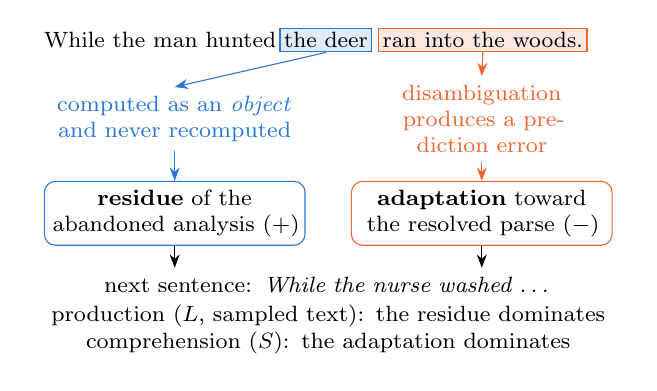
\begin{tikzpicture}[font=\footnotesize, >=Stealth, box/.style={text width=3.1cm, align=center, rounded corners, inner sep=3pt}]
\node[anchor=west, inner sep=1pt] (pre) at (0,0) {While the man hunted};
\node[anchor=west, inner sep=1.5pt, fill=gpblue!15, draw=gpblue] (np) at (pre.east) {the deer};
\node[anchor=west, inner sep=1.5pt, fill=gporange!15, draw=gporange] (mc) at ([xshift=2pt]np.east) {ran into the woods.};
\node[box, text=gpblue] (npl) at (1.7,-1.0) {computed as an \emph{object}\\ and never recomputed};
\node[box, text=gporange] (mcl) at (5.6,-1.0) {disambiguation produces a prediction error};
\draw[->, gpblue] (np.south) -- (npl.north);
\draw[->, gporange] (mc.south) -- (mcl.north);
\node[box, draw=gpblue] (r) at (1.7,-2.2) {\textbf{residue} of the abandoned analysis ($+$)};
\node[box, draw=gporange] (a) at (5.6,-2.2) {\textbf{adaptation} toward the resolved parse ($-$)};
\draw[->, gpblue] (npl) -- (r); \draw[->, gporange] (mcl) -- (a);
\node[text width=7.4cm, align=center] (t) at (3.65,-3.5) {next sentence: \emph{While the nurse washed \ldots}\\[1pt]
production ($L$, sampled text): the residue dominates\\ comprehension ($S$): the adaptation dominates};
\draw[->] (r.south) -- (r.south |- t.north); \draw[->] (a.south) -- (a.south |- t.north);
\end{tikzpicture}
\caption{Two traces of a garden-path sentence in a causal language model.
The states of \ex{the deer} are written under the object analysis and never revised (\S\ref{sec:mechanism}), and later text reads them as a residue of that analysis.
The main-clause states carry an adaptation toward the resolved structure.
The two traces push later processing in opposite directions, and the measure decides which one is visible (\S\ref{sec:twoforces}).}
\label{fig:schema}
\end{figure}

\section{Introduction}

Garden-path sentences make a reader build an analysis and then give it up.
In \ex{While the man hunted the deer ran into the woods}, the noun phrase \ex{the deer} is first attached as the object of \ex{hunted}, and the verb \ex{ran} reveals that it is the subject of the main clause \citep{frazier1982}.
Language models (LMs) have become a standard test bed for such sentences.
Their surprisal at the disambiguating word predicts that garden-path effects occur but underestimates how large they are \citep{futrell2019,vanschijndel2021,arehalli2022,huang2024}, and when asked \ex{Did the man hunt the deer?} they often answer yes, like human readers who keep part of the initial interpretation \citep{christianson2001,li2024incremental,amouyal2025}.
These studies examine the garden-path sentence itself, either the difficulty of its disambiguation or the accuracy of its final interpretation.

An abandoned analysis can also affect what comes after the sentence.
\citet{vangompel2006} had participants read a garden-path sentence and then complete a fragment such as \ex{While the nurse washed}.
Completions were more often transitive after the garden path than after a version disambiguated by a comma (33.6\% against 29.1\%), so the object analysis that had been ruled out still primed later production.
For LMs the same question bears on how they handle any interpretation that is revised within a context, from a misread instruction to a hypothesis abandoned in a reasoning trace.
A causal transformer computes the representation of each token once, when the token is read, and later tokens retrieve these representations by attention.
When the disambiguation arrives, the states of \ex{the deer} have already been computed under the object analysis, and nothing in the architecture revises them.

Work on structural priming in LMs offers two accounts of how a prime affects later text, and it has not been able to tell them apart.
LMs reuse the structure of a preceding sentence \citep{sinclair2022,michaelov2023,pucci2026}, and they do so more after less expected primes, an inverse-frequency effect that has been taken as evidence that in-context learning is error-driven \citep{jumelet2024,zhou2025icl}.
The alternative is residual activation, in which a processed structure stays available and is reused because it is active \citep{pickering1998}.
For an ordinary prime both accounts predict priming of the prime's structure, so all existing LM studies, which use unambiguous primes, are compatible with either.

Does an LM keep using an analysis it has abandoned?
A garden-path prime turns this question into a test between the two accounts \citep{chang2006,jaeger2013}.
Residual activation predicts priming of the abandoned object analysis.
Error-driven learning predicts the opposite, because the prediction error occurs when the object analysis fails, and learning from it should strengthen the resolved structure in which \ex{the deer} begins a new clause.
Human data show only the net of the two predictions.
An LM lets us measure both, and the architectural argument above leads to a concrete hypothesis about where a residue would come from.

We pair garden-path primes from five published item sets with target fragments and measure how the prime changes two quantities.
The first is production-like, the preference for attaching the target's noun phrase as an object, measured in log-probabilities and in sampled completions.
The second is comprehension-like, the surprisal of the disambiguating word in a garden-path target.
A contrast that matches primes for punctuation and verb isolates the effect of the abandoned analysis, and further controls replace the comma with case marking and remove the possibility of an object reading.
We test 24 models from six families between 124M and 70B parameters, fix the predictions of each confirmatory experiment before collecting its data, and use activation patching to locate the effects inside the prime.

The abandoned analysis persists in every model.
A garden-path prime raises later object attachment on discovery, held-out and human-normed items, on the discovery set by 76\% of the effect of a prime in which the noun phrase really is an object, and the residue appears in sampled completions.
The same prime drives an adaptation toward the resolved structure, which is causal within item families, grows with the prime's disambiguation error, and dominates the comprehension-like measure.
Patching shows that the two forces are read from different positions.
Replacing the states of \ex{the deer} with states computed under the subject analysis removes most of the residue, and all of it in the 32B and 70B models, whereas the states of the main clause carry the adaptation.
The paradigm also has to be adapted to LMs, because the raw statistic of the human study reverses in most models: they align with the punctuation of the prime and often write a garden-path sentence themselves.

Our contributions are as follows.
(1) We show that LMs carry an abandoned syntactic analysis into later production, across 24 models and three item sets, with controls for punctuation, verb bias, case and local string overlap.
(2) We show that a garden-path prime produces both a residue of the abandoned analysis and an error-driven adaptation toward the resolved one, with opposite signs, and that the measure determines which of them is observed, which gives a single case in which the residual-activation and error-driven accounts of priming are both at work.
(3) We locate the residue in noun-phrase states that a causal model computes before the disambiguation and never revises, and the adaptation in the states after it.
(4) We show that the human paradigm's statistic reverses in LMs because of punctuation alignment, and that question-answering measures of lingering misinterpretation are unrelated to the residue item by item.

\section{Related Work}

\paragraph{Garden paths in language models.}
Garden-path sentences were among the first constructions used to ask whether neural LMs track syntactic state \citep{futrell2019}.
Surprisal from such models predicts that the effects exist but underestimates their size and misorders constructions \citep{vanschijndel2021,arehalli2022,huang2024}, a gap that recent work attributes to how many parses a model keeps alive \citep{timkey2026} or closes with suitably trained models \citep{yoshida2026}.
Comprehension studies ask whether the final interpretation is correct.
LMs often accept the initial misreading, with plausibility and verb type modulating this as in humans \citep{li2024incremental,amouyal2025,amouyal2026}.
\citet{hanna2025} found features for both readings of a garden-path prefix in small models and showed that the circuit that answers comprehension questions hardly reuses them.
All of this work studies the garden-path sentence itself, and none asks what the abandoned analysis does to later text.

\paragraph{Structural priming and adaptation.}
In humans, recently processed structures are reused \citep{pickering1998}, and garden-path difficulty decreases with exposure \citep{fine2013}.
Two accounts explain such effects.
Residual activation holds that a processed structure remains active, and error-driven implicit learning holds that processing a prime adjusts expectations in proportion to its prediction error \citep{chang2006}, which predicts stronger priming from less expected primes \citep{jaeger2013}.
\citet{vangompel2006} found priming of the abandoned analysis of garden-path sentences, and \citet{fujita2020} found that unambiguous primes ease the reading of later garden paths without removing lingering misinterpretation.
In LMs, conditioning on a prime raises the probability of its structure in a target \citep{sinclair2022}, across languages \citep{michaelov2023} and in generation \citep{pucci2026}.
The effect is larger for less expected primes and with lexical overlap \citep{jumelet2024}, which \citet{zhou2025icl} take as evidence that in-context learning is a form of error-driven learning, and gradient updates on garden-path sentences improve the fit of RNN surprisal to human adaptation \citep{vanschijndel2018}.
These studies use unambiguous primes, for which the two accounts make the same prediction.

\paragraph{Revising interpretations in context.}
LMs rarely retract their own wrong answers, and the retractions they produce depend on internal belief representations \citep{yang2025retraction}, while self-correction without external feedback is unreliable \citep{kamoi2024}.
Mechanistic work shows that later tokens retrieve earlier bindings by attending back to the positions where they were encoded \citep{prakash2026}.
Activation patching, which replaces internal states with states from a counterfactual input, is the standard tool for locating such information \citep{vig2020causal,meng2022locating,zhang2024patching}.
Garden paths offer a controlled instance of revision, since the overridden interpretation, its strength and the point at which it is overridden are all known.

\section{Experimental Setup}
\label{sec:setup}

\paragraph{Materials.}
An item family is one garden-path sentence with its controls.
The discovery set contains 93 NP/Z families, 69 from \citet{amouyal2025} and 24 from the SAP benchmark \citep{huang2024}.
A held-out set of 48 families combines 24 items from \citet{cehakova2025} with 24 from SyntaxGym \citep{gauthier2020}, and was used only after the analyses had been fixed on the discovery set.
A third set contains the 54 items of \citet{christianson2001}, crossed with the length of the ambiguous region and the plausibility of the object reading.
Each family provides the prime conditions in Table~\ref{tab:conds}.
\cond{gp} is the garden-path sentence and \cond{cue} its version with a comma after the verb.
\cond{tb} replaces the main-clause subject with a pronoun, so that the noun phrase remains the object.
\cond{nb} and \cond{nc} replace the ambiguous verb with a strictly intransitive one, without and with the comma.
Further conditions are introduced with the experiments that use them.

\begin{table}[t]
\centering\small
\setlength{\tabcolsep}{3pt}
\begin{tabular}{lp{5.7cm}}
\toprule
Prime & Example\\
\midrule
\cond{gp} & While the man hunted the deer ran into the woods.\\
\cond{cue} & While the man hunted, the deer ran into the woods.\\
\cond{tb} & While the man hunted the deer it ran into the woods.\\
\cond{nb} / \cond{nc} & While the man slept(,) the deer ran into the woods.\\
\cond{nom} & While the man hunted they ran into the woods.\\
\cond{pass} & While the man was hunted the deer ran into the woods.\\
\midrule
Target & Quantity\\
\midrule
$L$ & $\log P(\text{\ex{\ldots washed the baby,}}) - \log P(\text{\ex{\ldots washed, the baby}})$\\
$S$ & $-\log P(\text{\ex{cried}} \mid \text{\ex{While the nurse washed the baby}})$\\
$G$ & sampled continuation of \ex{While the nurse washed}\\
\bottomrule
\end{tabular}
\caption{Prime conditions and target quantities, illustrated with one prime and one target family. \cond{nom} and \cond{pass} are used only in the experiments that test punctuation and local coherence (\S\ref{sec:residue}).}
\label{tab:conds}
\end{table}

\paragraph{Targets and measures.}
Each prime is followed by a target from every other family that shares no content word with it, so in the discovery set each prime is measured against 78 to 92 targets.
For a target family with subject $s$, verb $v$ and noun phrase $n$, the production-like measure is
\begin{equation}
L = \log P(\text{\ex{While}}\ s\ v\ n\text{,}) - \log P(\text{\ex{While}}\ s\ v\text{,}\ n),
\end{equation}
where both probabilities are conditioned on the prime.
$L$ is the log-odds of attaching $n$ as the object of $v$ rather than starting a new clause with it.
The comprehension-like measure $S$ is the surprisal of the first word of the target's main clause after the comma-less fragment \ex{While}~$s$~$v$~$n$.
A high $S$ means that the model expected $n$ to be an object, so both $L$ and $S$ increase with object attachment.
For sampled production we let the model continue \ex{While}~$s$~$v$ and code whether the continuation attaches a noun phrase as an object, with a rule system over part-of-speech tags that is correct on 99.7\% of 1,066 sentences of known structure (Appendix~\ref{app:coding}).

\paragraph{The residue contrast.}
Comparing \cond{gp} with \cond{cue} confounds the abandoned analysis with the comma, and comparing \cond{gp} with \cond{nb} confounds it with the verb.
For any measure $X$ we use
\begin{equation}
A_X = \big(X_{\cond{gp}} - X_{\cond{nb}}\big) - \big(X_{\cond{cue}} - X_{\cond{nc}}\big),
\label{eq:A}
\end{equation}
where $X_c$ is the mean of $X$ over targets after primes of condition $c$.
Within each bracket the two primes have the same punctuation, and across brackets the same verbs, so $A_X$ measures what is specific to a comma-less prime with a transitive verb, which is the condition under which the object analysis is first built and then abandoned.
The same contrast with \cond{tb} in place of \cond{gp} gives the effect of a prime whose noun phrase really is an object, and we report the residue relative to it as $r = A_X/A_X^{\cond{tb}}$.

\paragraph{Models and inference.}
We use 24 open-weight causal LMs from the GPT-2, Pythia, Llama, Mistral, Gemma and Qwen families, base and instruction-tuned, between 124M and 70B parameters and including one mixture-of-experts model (Appendix~\ref{app:models}).
Scoring uses exact log-probabilities without chat templates, and sampled completions use temperature 1 with no truncation.
Primes and targets are both random factors, so intervals come from a two-way bootstrap that resamples prime families and target families independently.
Summaries across models use random-effects meta-analysis \citep{dersimonian1986}.
For every confirmatory experiment we fixed the predictions and the analysis in a dated record before collecting its data, and Appendix~\ref{app:prereg} lists all outcomes.

\begin{figure*}[t]
\centering
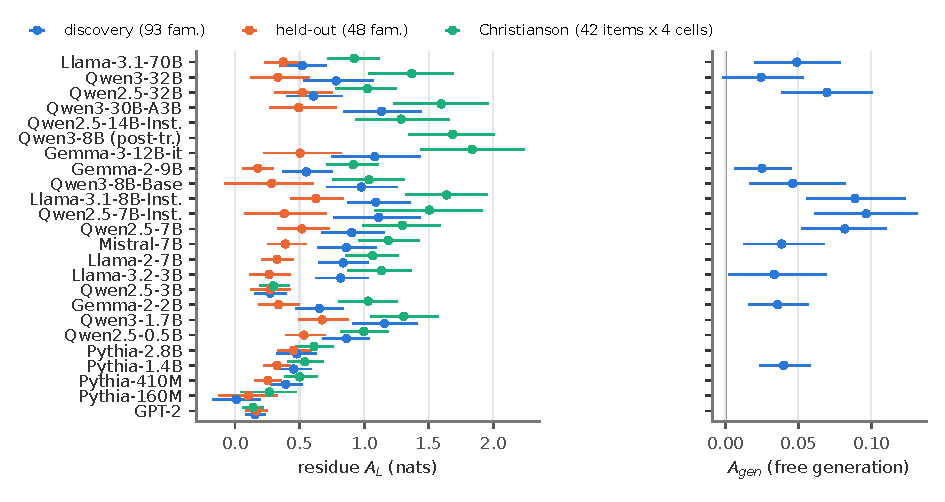
\includegraphics[width=\textwidth]{figures/fig_residue}
\caption{The residue of the abandoned object analysis in every model. Left: $A_L$ (Eq.~\ref{eq:A}) per model on the discovery, held-out and \citet{christianson2001} item sets. Right: the same contrast on sampled completions, as a difference in the proportion of transitive continuations. Error bars are 95\% intervals from a two-way bootstrap over prime and target families. Models are ordered by size.}
\label{fig:residue}
\end{figure*}

\section{The Abandoned Analysis Persists}
\label{sec:residue}

\paragraph{The residue in production.}
After a garden-path prime, all 24 models prefer object attachment in the target more than the controls predict (Figure~\ref{fig:residue}).
On the discovery set $A_L$ is positive in 22 of 22 models and its interval excludes zero in 21, with a pooled value of 0.70 nats, which is 76\% of the effect of a prime in which the noun phrase really is the object.
The residue replicates on the held-out families, where it is positive in all 22 models with a median of 0.36 nats, and on the human-normed items of \citet{christianson2001}, where it is positive in all 24 models with a median of 1.05 nats.
Its size varies between models without a monotonic relation to model size, and the 70B model shows a residue of 0.52 nats.

\paragraph{Punctuation.}
A comma-less prime is unusual in written English, and models adapt to this property.
After an \cond{nb} prime, which contains no ambiguity but omits the comma, a later comma-less garden-path resolution is less surprising than after \cond{nc} in all 22 models, by 2.8 nats on average.
Equation~\ref{eq:A} subtracts this adaptation, and a separate experiment removes punctuation as a disambiguator altogether.
In \cond{nom} the nominative pronoun \ex{they} rules out the object reading while the verb and the missing comma stay the same as in \cond{gp}.
Across families, the residue then still rises with the model's expectation of an object after the ambiguous verb, in 22 of 22 models (16 individually significant).

\paragraph{An entertained analysis.}
The string \ex{hunted the deer} could prime object attachment by local coherence alone, as it does for human readers \citep{tabor2004}.
In \cond{pass} the same string appears in a passive clause, where \ex{the deer} cannot be an object.
Across 22 models the residue of \cond{pass} has a median of 12\% of the \cond{gp} residue, and it is reliably negative in seven, mostly small, models.
The residue requires that the object analysis was licensed when the noun phrase was read.
The ratio rises in the strongest models, to 0.45 in Llama-3.1-70B and above 0.5 in the two Qwen2.5-7B models, so that in these models a locally computed object reading also leaves a trace.

\paragraph{Sampled production.}
Log-probabilities of two fixed strings may not reflect what a model writes, so we sampled two continuations of every target fragment after every prime in 12 models, about 57,000 prompts per model.
The residue appears in the proportion of transitive continuations in 11 of 12 models, with a pooled value of 5.0 percentage points (Figure~\ref{fig:residue}, right), and its size across models follows $A_L$ (Spearman $\rho=0.81$ in the first eight models).
Relative to a real object prime, the residue is smaller in sampled text (about 20\%) than in $L$ (\S\ref{sec:transfer}).

\section{Two Forces with Opposite Signs}
\label{sec:twoforces}

\begin{figure*}[t]
\centering
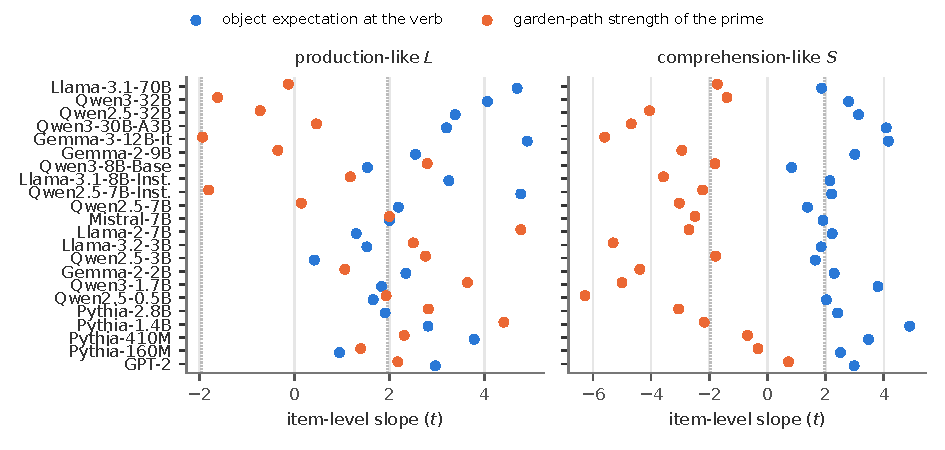
\includegraphics[width=\textwidth]{figures/fig_slopes}
\caption{Item-level predictors of the residue $A$ on the discovery set, per model. Each point is the $t$ value of a predictor in a regression of family-level $A$ on the model's object expectation after the ambiguous verb (blue) and on the garden-path strength of the prime, the surprisal of its disambiguating word without versus with the comma (orange). Dotted lines mark $|t|=1.96$. Object expectation raises $A$ on both measures. Garden-path strength lowers it on the comprehension-like measure $S$ in 21 of 22 models.}
\label{fig:slopes}
\end{figure*}

The residue is not the only effect of a garden-path prime.
On the comprehension-like measure $S$ the contrast $A_S$ is close to zero on average (0.05 nats over 22 models) and varies in sign, significantly positive in five models and significantly negative in four.
A negative value means that after a garden-path prime the model expects an object less than the controls predict, which is an adaptation toward the structure the prime turned out to have.

\paragraph{Two predictors with opposite effects.}
The two accounts of priming tie the effect of a prime to different properties.
Residual activation depends on how strongly the abandoned analysis was built, which we measure as the model's expectation of an object after the ambiguous verb, $\log P(\text{\ex{the}}) - \log P(\text{\ex{,}})$.
Error-driven learning depends on the prediction error at the disambiguation, which we measure as the garden-path strength of the prime, the surprisal of its disambiguating word without the comma minus that with the comma.
Figure~\ref{fig:slopes} regresses the family-level residue on both.
Object expectation raises the residue on both measures in all 22 models.
Garden-path strength lowers it on $S$ in 21 of 22 models (15 individually significant), and on $L$ it has the opposite sign in most models, so in 21 of 22 models its effect is more negative on $S$ than on $L$.
A prime carries both forces, and their balance differs between the two measures.

\paragraph{The error force is causal.}
Garden-path strength varies between families together with many other properties.
To manipulate it within a family, we kept each prime up to the noun phrase fixed, which fixes the object analysis that the model builds, and varied only the continuation, which changes the surprisal at the disambiguation.
More surprising disambiguations reduce the residue on $S$ within families, with $t$ values between $-4.1$ and $-6.4$ in the three models whose between-family analysis had shown an error effect, and close to zero in the two models whose between-family analysis had shown none.
The surprisal summed over the whole continuation predicts little, so the relevant error is the one at the point of disambiguation (Appendix~\ref{app:prereg}).
On the items of \citet{christianson2001}, plausibility changes only the main-clause continuation, which allows the same within-family test on human-normed material, and there the error effect is negative in 10 of 10 models that pass the comprehension controls.

\paragraph{The residue grows with the abandoned analysis.}
A context sentence before the prime that makes the noun phrase a likely object (\ex{The man had been tracking the deer since dawn.}) strengthens the garden path by 0.9 to 1.7 nats in all 11 models we tested.
It raises the residue on $S$ in 10 of 11 models, 8 of them significantly, although the stronger garden path also means a larger disambiguation error, which on an error-only account would lower it.
The check we had specified for this experiment, a change in object expectation at the verb, was not met, so we treat this result as converging evidence (Appendix~\ref{app:e014}).
The direct test of the residue is the patching experiment of \S\ref{sec:mechanism}.

\paragraph{The measure decides which force is seen.}
The residue dominates the production-like measure, and the adaptation dominates the comprehension-like one.
We tested this pattern prospectively on the items of \citet{christianson2001}, which were not used to discover it.
The residue on $L$ was positive in 16 of 16 models, and the error effect was more negative on $S$ than on $L$ in 14 of 16.
The human literature contains the same two forces in separate paradigms, priming of the abandoned analysis in production \citep{vangompel2006} and adaptation to garden paths in comprehension \citep{fine2013}.
In LMs both arise from the same prime.

\paragraph{Scope.}
With the same pre-specified analysis, the two forces do not appear for NP/S garden paths (\ex{The man knew the answer was wrong}), and the error force appears for main-verb/reduced-relative garden paths in six of nine models.
NP/Z and main-verb/reduced-relative ambiguities both require the reader to undo an attachment, whereas NP/S reanalysis only adds structure to the analysis already built \citep{sturt1996}, so the two forces appear to be specific to reanalysis that destroys a committed structure.

\section{Where the Residue Lives}
\label{sec:mechanism}

A causal transformer computes the states of \ex{the deer} before it reaches \ex{ran}.
In the garden-path prime these states are identical to those of the transitive prime \cond{tb}, since the two share every preceding token, and later tokens, including those of the next sentence, attend to keys and values built under the object analysis.
If the residue is read from these stale states, replacing them with states computed under the subject analysis should remove it.
The alternative is that the residue is read from the main clause, whose states processed the disambiguation and could encode the reanalysis.

\paragraph{Patching design.}
We construct a counterfactual prime in which the noun phrase was analysed as a subject from the start.
At every layer, the residual-stream states of the noun-phrase tokens in \cond{gp} are replaced with the states of the same tokens in \cond{cue}, where the comma has already made the noun phrase a subject, and the rest of the prime is recomputed.
The target then attends to a mixture of the original and the counterfactual prime.
In the NP condition it reads counterfactual keys and values at the noun phrase and original ones elsewhere, in the MC condition counterfactual ones at the main clause (\ex{ran into the woods.}), and in the full condition both.
The same procedure applied to \cond{nb} with \cond{nc} as donor estimates what the replacement does merely by importing information about the comma, and Equation~\ref{eq:A} subtracts it.
We report the retained residue $\rho = A_L^{\text{patched}}/A_L$ on the production-like measure and the change $\Delta = A_S^{\text{patched}} - A_S$ on the comprehension-like measure, for nine models between 1.4B and 70B parameters.

\begin{figure}[t]
\centering
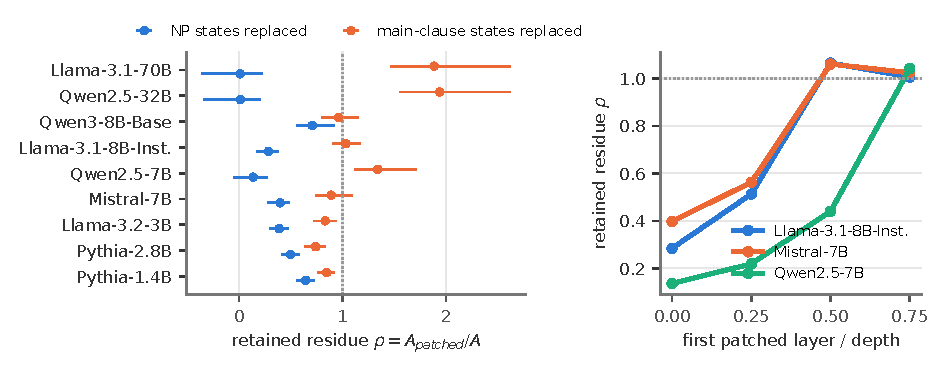
\includegraphics[width=\columnwidth]{figures/fig_patching}
\caption{Patching the garden-path prime. Left: residue on $L$ retained when the target reads counterfactual subject-analysis states at the noun phrase (blue) or at the main clause (orange). Right: noun-phrase states replaced only from a given fraction of the network's depth onward. Values and intervals for both measures are in Appendix~\ref{app:patching}.}
\label{fig:mech}
\end{figure}

\paragraph{The noun phrase carries the residue.}
Replacing the noun-phrase states removes most of the residue (Figure~\ref{fig:mech}, left).
The retained fraction ranges from 0.71 to 0.01, with a pooled value of 0.37, and in Qwen2.5-32B and Llama-3.1-70B the residue disappears.
Replacing the main-clause states leaves it intact on average (pooled $\rho=1.01$), and the noun phrase carries more of the residue than the main clause in all nine models.
The effect does not come from the comma of the donor: when the donor is \cond{nb}, in which the noun phrase follows an intransitive verb without a comma, the retained fraction is 0.34 to 0.46 in the three models tested.
Replacing the noun-phrase states only in the upper half of the network has no effect in Llama-3.1-8B-Instruct and Mistral-7B, and replacing them in the upper quarter has none in Qwen2.5-7B (Figure~\ref{fig:mech}, right), so the next sentence reads the abandoned analysis from the lower and middle layers, where the noun phrase's syntactic role is computed.

\paragraph{The main clause carries the adaptation.}
On the comprehension-like measure the two parts of the prime act in opposite directions in all nine models.
Replacing the noun-phrase states lowers $A_S$ by 0.26 to 1.11 nats, removing the residue's positive contribution, and replacing the main-clause states raises it by 0.22 to 2.00 nats, removing the adaptation.
The two forces of \S\ref{sec:twoforces} are read from different positions of the same prime.
In the larger models the main-clause replacement also raises the residue on $L$, to 1.34 times its original value in Qwen2.5-7B and 1.9 times in Qwen2.5-32B and Llama-3.1-70B, so that even on the production-like measure the observed residue is reduced by the adaptation, and the persistence of the abandoned analysis is larger than the net effect shows.

\section{Transferring the Human Paradigm}
\label{sec:transfer}

\begin{figure}[t]
\centering
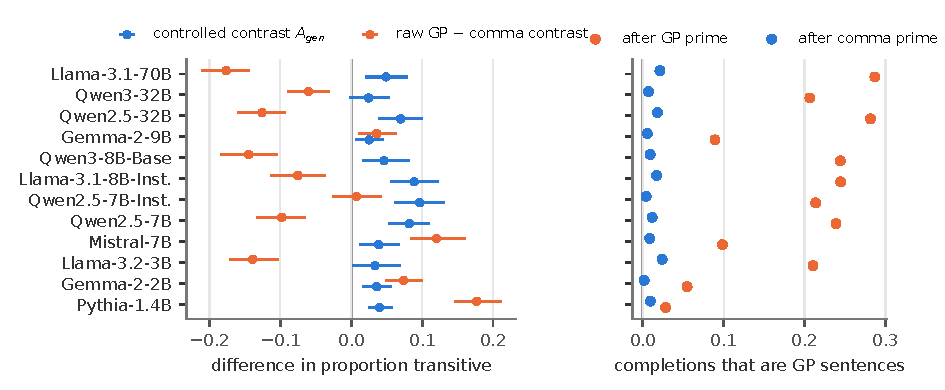
\includegraphics[width=\columnwidth]{figures/fig_generation}
\caption{Sampled production. Left: the controlled residue $A$ (blue) and the raw contrast between garden-path and comma primes used in the human study (orange). Right: proportion of completions that are themselves comma-less garden-path sentences, after a garden-path prime (orange) and after a comma prime (blue).}
\label{fig:generation}
\end{figure}

\paragraph{The raw statistic reverses.}
The human study compared completions after \cond{gp} and \cond{cue} primes.
In LMs this contrast is reliably positive in only 4 of 12 models and significantly negative in 7 of the 8 Llama and Qwen models, most strongly in Llama-3.1-70B, where garden-path primes lower the proportion of transitive completions by 17.6 points (Figure~\ref{fig:generation}, left).
The completions show why.
After a garden-path prime, up to 29\% of the completions are themselves comma-less garden-path sentences, against 0.2\% to 2.4\% after a comma prime, in all 12 models (Figure~\ref{fig:generation}, right).
A model that has just read a sentence without the expected comma writes one, and since the raw contrast counts these completions as intransitive, it mixes the residue with this stylistic alignment.
Participants in the human study completed fragments aloud, where punctuation plays no role.
The contrast of Equation~\ref{eq:A} matches primes for punctuation, and with it the residue is positive in 11 of 12 models.
The same alignment explains why the residue is smaller in sampled text than in $L$, which compares two strings with identical words and fixed punctuation.

\paragraph{Lingering comprehension is a separate phenomenon.}
LMs answer \ex{Did the man hunt the deer?} with yes after the garden-path sentence much more often than after its comma version, and more so when the ambiguous region is longer, as human readers do \citep{christianson2001}.
This lingering misinterpretation could be another expression of the residue.
On the items of \citet{christianson2001} it is not, since across items its correlation with the priming residue lies between $-0.30$ and $0.15$ in the ten models that pass the comprehension controls, although both measures are reliable (split-half reliabilities of 0.77 to 0.98).
A context sentence that restates the main clause reduces lingering in seven of seven models, whereas a reordered paraphrase that removes the garden path more completely reduces it less, so lingering does not follow the garden-path processing in the way the residue does.
Studies that measure lingering in LMs by question answering \citep{li2024incremental,amouyal2025} and the residue measured here describe different properties of the model.

\section{Discussion and Conclusion}

Garden-path primes separate two accounts of priming that ordinary primes cannot, and in LMs both accounts describe part of what happens.
The residue of the abandoned analysis follows the strength of that analysis and is read from the positions where it was built.
The adaptation follows the prediction error and is read from the positions where the error occurred.
This yields a prediction for human readers.
If the same superposition holds in people, garden paths with a more surprising disambiguation should produce less priming of the abandoned analysis in production and more adaptation in comprehension, which can be tested by combining the paradigm of \citet{vangompel2006} with cloze norms for the disambiguating word.

Neither force is confined to small or base models.
The residue is positive in all 22 models of the discovery set and reliably so in all except Pythia-160M, which together with GPT-2 has the weakest garden-path effect of the panel.
Instruction tuning does not remove it, and the three instruction-tuned models show the largest residues (1.08 to 1.11 nats, against 0.90 for the base version of Qwen2.5-7B).
Model size mainly shifts the balance between the two forces.
In the 32B and 70B models the residue is confined to the noun phrase more completely than in smaller ones, and their main-clause adaptation is strong enough to hide about half of the residue on the production-like measure.

For LMs, the residue has a concrete source.
In human processing, residual activation names a memory trace of unknown substrate.
In a causal transformer, representations are written when each token is read, and later tokens consult them through attention without revising them.
A reanalysis can change what later positions compute, but it cannot change what earlier positions hold, and our patching results show that later text reads the abandoned analysis from there.
This adds a qualification to the view that in-context learning is error-driven \citep{zhou2025icl}.
The error force we find fits that view, but an error-driven learner would not reuse the analysis that was rejected, and the residue shows that context effects in LMs also include persistence of representations that the error signal has already overruled.
The same argument applies to any interpretation that a model builds and later revises within its context, such as a misread instruction or a hypothesis abandoned during reasoning, and garden paths provide a case in which the abandoned interpretation and the moment of its revision are known exactly.

\section*{Limitations}

We study English garden paths, mostly of the NP/Z type, and use NP/S and main-verb/reduced-relative sentences only to delimit the scope of the two forces.
Other languages and other kinds of temporary ambiguity may behave differently.
Our models are open-weight models up to 70B parameters, because the analyses require exact log-probabilities and access to internal states, and closed models were not tested.
The behavioural manipulation of the abandoned analysis (Appendix~\ref{app:e014}) did not pass its pre-specified check, so the causal evidence for the residue comes from activation patching, and patching was run on nine of the 24 models.
The contrast of Equation~\ref{eq:A} was defined after inspecting the first two models of the discovery set, and its confirmation rests on held-out items, a prospective test and pre-specified predictions, some of which failed (Appendix~\ref{app:prereg}).
The coding of sampled completions is rule-based and was checked against gold sentences and by one annotator on a sample of generations.
We derive a prediction for human readers but do not test it.

\section*{Ethical Considerations}

This work involves no human participants and no personal data.
All models are public checkpoints used for scoring and sampling on local hardware.
The materials come from published studies and benchmarks and are used for research with citation.

\bibliography{refs}

\appendix

\section{Models}
\label{app:models}

Table~\ref{tab:models} lists the 24 models.
All weights are public Hugging Face checkpoints: GPT-2 \citep{radford2019language}, Pythia \citep{biderman2023pythia}, Llama~2 and Llama~3 \citep{touvron2023llama,grattafiori2024llama}, Mistral \citep{jiang2023mistral}, Gemma~2 and Gemma~3 \citep{gemma2024gemma2,gemma2025gemma3}, Qwen2.5 \citep{qwen2024qwen25} and Qwen3 \citep{yang2025qwen3}.
Pythia-410M is the seed-1 checkpoint of the Pythia suite.
Log-probabilities are computed on the jointly tokenized prime and target, with the prime preceded by the beginning-of-sequence token and separated from the target by a space.
A target token counts toward the continuation if its character span starts at or after the continuation's first character.
Priming scores were computed in bfloat16.
Patching runs used float32 for models up to 8B parameters, where the cached and the full-sequence computations agree to $10^{-4}$ nats, and bfloat16 for Qwen2.5-32B and Llama-3.1-70B, which ran on two GPUs.
Sampled completions were generated with vLLM \citep{kwon2023vllm} using temperature 1, top-$p$ 1, at most 24 new tokens and a stop at the first line break.

\begin{table*}[t]
\centering\footnotesize
\setlength{\tabcolsep}{3pt}
\begin{adjustbox}{max width=\textwidth}
\begin{tabular}{lllcccccccc}
\toprule
Model & Size & Type & Disc. & Held-out & \cond{nom} & \cond{pass} & Christianson & Sampled & Patching & Context\\
\midrule
\rows{tables/models.tex}
\bottomrule
\end{tabular}
\end{adjustbox}
\caption{The 24 models and the experiments they enter. Disc.: discovery set (\S\ref{sec:residue}, \S\ref{sec:twoforces}). Held-out: 48 held-out families. \cond{nom}: case disambiguation. \cond{pass}: passive primes. Christianson: items of \citet{christianson2001}, used for the prospective test of \S\ref{sec:twoforces} and for comprehension questions (\S\ref{sec:transfer}). Sampled: sampled completions. Patching: \S\ref{sec:mechanism}. Context: Appendix~\ref{app:e014}.}
\label{tab:models}
\end{table*}

\section{Materials}
\label{app:materials}

The discovery families come from the released items of \citet{amouyal2025} and from the NP/Z subset of the SAP benchmark \citep{huang2024}.
For each family we wrote the comma version (\cond{cue}), the transitive versions with a resumptive pronoun (\cond{tb}, \cond{tc}), and the two intransitive versions (\cond{nb}, \cond{nc}).
The intransitive verbs (\ex{slept, yawned, sneezed, laughed, sighed, snored, napped, shivered, dozed, frowned, giggled, rested}) cannot take an object, and each family uses one of them with the family's own subject.
The held-out families combine 24 items with reflexive-absolute verbs from \citet{cehakova2025} with 24 NP/Z items from SyntaxGym \citep{gauthier2020}.
The two sources differ in the object expectation of their verbs (about $-0.3$ and $1.5$ nats on average), which is why we report between-family slopes on the held-out set with source fixed effects.
The items of \citet{christianson2001} were transcribed from the published appendix.
They comprise 42 optionally transitive and 12 reflexive-absolute verbs, each with a short and a long ambiguous region (\ex{the deer} against \ex{the deer that was brown and graceful}) and, for the optionally transitive verbs, a plausible and an implausible object.
Primes from this set are followed by a fixed set of 48 discovery families as targets, excluding any target that shares a content word with the prime.

A target never shares a content word with its prime, which removes lexical repetition as a source of priming.
In the discovery set each prime is paired with 78 to 92 targets.
The $L$ measure compares two strings that contain the same words in the same order and differ only in the position of the comma.
The $S$ measure scores only the first word of the main clause, so its value does not depend on the length of the continuation.

\section{Statistics}
\label{app:stats}

For a model and a contrast, we first average the measure over targets for every prime family and condition, then average over prime families.
Intervals resample prime families and target families independently with replacement (1,000 draws) and recompute the contrast, which treats both as random samples of items.
Item-level regressions (Figure~\ref{fig:slopes}) regress the family-level contrast on the two standardized predictors with heteroskedasticity-consistent standard errors.
Across models we pool per-model estimates with the random-effects estimator of \citet{dersimonian1986}, taking the standard error of each model's estimate from its bootstrap interval.
Models are not a random sample of language models, so we read the pooled value as the typical model of our panel and always report how many models show the effect.
Table~\ref{tab:residue} gives the residue of every model on the three item sets, and Figure~\ref{fig:slopes} the item-level regressions of \S\ref{sec:twoforces}.

\begin{figure*}[t]
\centering
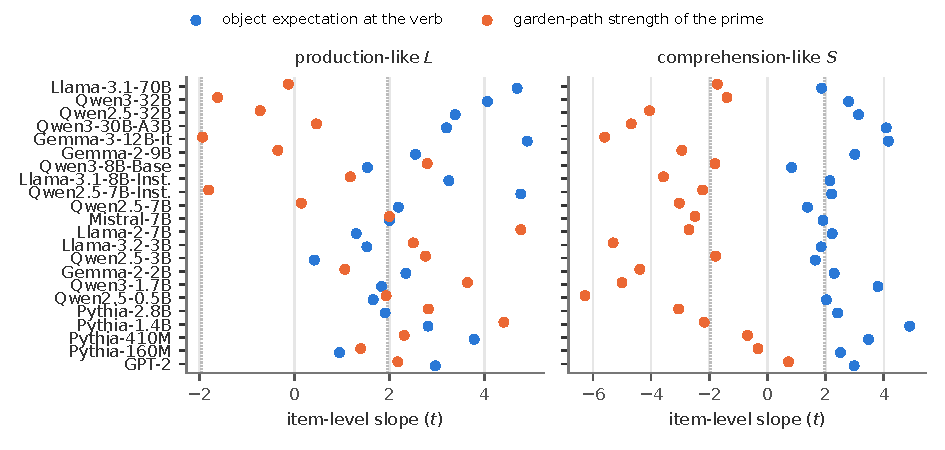
\includegraphics[width=\textwidth]{figures/fig_slopes}
\caption{Item-level predictors of the residue on the discovery set. Each point is the $t$ value of one predictor in a regression of the family-level contrast $A$ on the model's object expectation after the ambiguous verb (blue) and on the garden-path strength of the prime, the surprisal of its disambiguating word without versus with the comma (orange). Dotted lines mark $|t|=1.96$. Object expectation raises $A$ on both measures. Garden-path strength lowers it on the comprehension-like measure $S$ in 21 of 22 models.}
\label{fig:slopes}
\end{figure*}


\begin{table}[t]
\centering\footnotesize
\setlength{\tabcolsep}{2pt}
\begin{adjustbox}{max width=\columnwidth}
\begin{tabular}{lccc}
\toprule
Model & Discovery & Held-out & Christianson\\
\midrule
\rows{tables/residue_sets.tex}
\bottomrule
\end{tabular}
\end{adjustbox}
\caption{Residue $A_L$ (nats) with 95\% two-way bootstrap intervals on the three item sets. Dashes mark models not run on a set.}
\label{tab:residue}
\end{table}

\section{Pre-specified Predictions and Outcomes}
\label{app:prereg}

Each confirmatory experiment was preceded by a dated record of its design, predictions and analysis, committed to version control before any of its data were collected.
Table~\ref{tab:prereg} lists every prediction and its outcome.
Three experiments did not confirm what we expected.
On the held-out families, the between-family relation between object expectation and the residue was measured on $S$ and was confirmed in only 6 of 15 models, whereas the error relation was confirmed in 9 of 15.
Figure~\ref{fig:slopes} shows that object expectation predicts the residue on both measures within the discovery set, and the held-out result indicates that the relation is weaker on $S$ when the families come from sources that differ in verb class.
For NP/S garden paths neither force appeared, which led to the scope statement of \S\ref{sec:twoforces}.
The context manipulation of Appendix~\ref{app:e014} failed its manipulation check.

The within-family manipulation of the error used continuations generated to follow each fixed prefix and checked for grammaticality.
Each family had between four and eight continuations whose disambiguating words differed in surprisal.
The effect of the error remained when only human-written continuations were used, when a naturalness score of the continuation was added as a covariate, and when continuations beginning with an auxiliary were removed ($t$ between $-2.8$ and $-6.2$ in the three models with an error effect).

\begin{table*}[t]
\centering\small
\setlength{\tabcolsep}{4pt}
\begin{tabular}{p{2.6cm}p{6.6cm}p{5.6cm}}
\toprule
Experiment & Pre-specified prediction & Outcome\\
\midrule
Held-out families & (i) object expectation predicts the residue on $S$ (ii) error predicts it with the sign found in discovery (iii) sign of the net residue & (i) 7/17 \emph{(not confirmed)} (ii) 11/17, same sign in 16/17 (sign test $p=.0001$) (iii) 5/9\\
Within-family error & more surprising disambiguation lowers the residue in the models with a discovery error effect & confirmed in 3/3, and null in the 2 models predicted null\\
NP/S & the two forces generalize to NP/S garden paths & \emph{not confirmed} (1/5 and 0/4)\\
MV/RR & error and commitment relations in main-verb/reduced-relative garden paths & (i) error 6/9 (ii) commitment 0/8\\
Case (\cond{nom}) & (i) object expectation predicts the residue without punctuation (ii) error relation negative (iii) comma part of the predictor vanishes & (i) 22/22 (ii) 20/22 (iii) \emph{not confirmed} (reinterpreted as part of object expectation)\\
Measures & (i) residue on $L$ positive (ii) error relation stronger on $S$ than on $L$ & (i) 16/16 (ii) 14/16\\
Passive (\cond{pass}) & passive residue small relative to \cond{gp} & median ratio 0.12 (confirmed)\\
Sampled text & (i) residue positive (ii) raw \cond{gp}$-$\cond{cue} contrast positive (iii) style alignment (iv) size follows $A_L$ & (i) 11/12 (ii) \emph{4/12} (iii) 12/12 (iv) $\rho=0.81$\\
Patching & (i) NP retains $\le 50\%$ and less than MC on $L$ (ii) MC changes $S$ more than NP & (i) 7/9 (ii) 8/9\\
Context & manipulation check on object expectation at the verb & \emph{not met} (0/11)\\
\bottomrule
\end{tabular}
\caption{Pre-specified predictions and outcomes. Counts are models in which the prediction held. Outcomes that did not confirm the prediction are in italics.}
\label{tab:prereg}
\end{table*}

\section{Patching}
\label{app:patching}

For a prime with noun-phrase tokens $N$ and main-clause tokens $M$, we run the prime twice.
The original run keeps all states.
The counterfactual run overwrites, at the output of every layer, the residual-stream vectors at $N$ with the vectors of the same tokens from the donor prime, and recomputes all positions after $N$ with these vectors in place.
Since the models use rotary position embeddings, the residual stream carries no absolute position, and the one-token offset introduced by the donor's comma does not need correction.
The target is then scored against a key--value cache that takes the counterfactual run's keys and values at the positions of the chosen span and the original run's elsewhere.
The prediction of the target's first token comes from the run that supplies the prime's last token.
Table~\ref{tab:patching} gives all estimates with intervals.
In the depth analysis the overwrite starts at layer $\lfloor fL \rfloor$ for $f \in \{0.25, 0.5, 0.75\}$, so that the noun phrase's keys and values below that layer keep the object analysis.
The retained fractions when the overwrite starts at a quarter, half and three quarters of the depth are 0.51 (0.41, 0.61), 1.07 (1.01, 1.12) and 1.01 (1.00, 1.01) for Llama-3.1-8B-Instruct, 0.56 (0.45, 0.65), 1.06 (1.02, 1.12) and 1.02 (1.01, 1.04) for Mistral-7B, and 0.22 (0.02, 0.35), 0.44 (0.28, 0.55) and 1.04 (1.01, 1.08) for Qwen2.5-7B.
Replacing both the noun phrase and the main clause retains 0.32 to 0.67 of the residue, more than replacing the noun phrase alone, because it also removes the adaptation.
For the role direction we take, at each layer, the difference between the mean noun-phrase states of object primes without a comma (\cond{tb}) and subject primes without a comma (\cond{nb}), fit without the prime's own family.
In the middle half of the layers the projection of the noun-phrase states on this direction is set to the subject mean, and the same shift along three norm-matched random directions serves as control.
The residue retained is 0.50 to 0.92 with the role direction and 0.42 to 0.83 with random directions, and the role direction retains less in Llama-3.2-3B, Llama-3.1-8B-Instruct and Qwen2.5-32B.
A direction fit on object primes against subject primes with a comma retains 0.31 to 0.74, less than random directions in all seven models, but it also separates primes with and without a comma.

\begin{table*}[t]
\centering\small
\setlength{\tabcolsep}{4pt}
\begin{tabular}{lccccc}
\toprule
Model & $A_L$ & $\rho$, NP & $\rho$, MC & $\Delta A_S$, NP & $\Delta A_S$, MC\\
\midrule
\rows{tables/e013_ci.tex}
\bottomrule
\end{tabular}
\caption{Patching results with 95\% two-way bootstrap intervals. $\rho$: retained fraction of the residue on $L$. $\Delta A_S$: change of the residue on $S$ in nats. NP and MC: the target reads counterfactual states at the noun phrase or at the main clause.}
\label{tab:patching}
\end{table*}

\section{Context Manipulation}
\label{app:e014}

Each of 87 discovery families received five context sentences, written by Qwen3-32B from a fixed instruction and checked automatically for length, the absence of commas, and the absence of the family's verbs and main-clause words.
Two contexts present the noun phrase as the subject's goal (\ex{The man had been tracking the deer since dawn.}), two present the subject and the noun phrase as doing unrelated things (\ex{The man studied the map while the deer drifted downstream.}), and one only places them together.
Six families for which no context passed the checks were dropped as specified.
Each context precedes all four primes of Equation~\ref{eq:A}, so the context's direct effect on the target cancels.

The specified manipulation check required object expectation after the ambiguous verb to be higher after goal contexts in more than 70\% of families.
It rose on average in every model but in only 48\% to 64\% of families, so the confirmatory test is uninformative by its own criterion.
The contexts did change the garden path itself: the surprisal of the disambiguating word without versus with the comma rose by 0.9 to 1.7 nats (Table~\ref{tab:e014}).
This analysis was added after the first two models had been scored.
Under it, the residue on $S$ is larger after goal contexts in 10 of 11 models, which runs against an account in which the prime acts only through its disambiguation error, since that error also grows.

\begin{table}[t]
\centering\footnotesize
\setlength{\tabcolsep}{2.5pt}
\begin{adjustbox}{max width=\columnwidth}
\begin{tabular}{lccccc}
\toprule
Model & $\Delta$exp. & fam. & $\Delta$GP & $\Delta A_L$ & $\Delta A_S$\\
\midrule
\rows{tables/e014.tex}
\bottomrule
\end{tabular}
\end{adjustbox}
\caption{Context manipulation, goal minus unrelated contexts. $\Delta$exp.: object expectation at the verb (pre-specified check), and the share of families in which it rose. $\Delta$GP: garden-path strength. $\Delta A_L$, $\Delta A_S$: change of the residue, with standard errors over families.}
\label{tab:e014}
\end{table}

\section{Overridden Statements}
\label{app:facts}

The 200 items combine ten frames (meeting day, location of objects, city of residence, start time, favourite colour, due month, profession, material, instrument, language) with five entities and two pairs of values in both orders.
Every context starts with a short label (\ex{Note:}, \ex{Mistake:}), so that the overridden statement is tokenized identically in all conditions.
The measure is $M=\log P(A)-\log P(B)$ after the probe, and $R=M_{\text{CORR}}-M_{\text{CTRL}}$.
In the re-encoding test, the residual-stream states of the overridden statement's tokens in CORR are replaced at every layer by those of the same tokens in PRE, where \ex{Mistake:} precedes the statement, and the same replacement in CTRL is subtracted.
This leaves the pull largely intact (Table~\ref{tab:facts}), as the pre-specified prediction did not expect.
The knockout analysis uses full sequences with a four-dimensional attention mask that blocks the listed query--key pairs in every layer and head.
Retained fractions of the pull, for blocking the answer's access to the statement, the answer's access to the value token only, and all later positions' access to the statement, are 1.10, 0.94, 0.12 (Llama-3.2-3B); 1.64, 1.53, 0.21 (Llama-3.1-8B-Instruct); 1.34, 1.10, $-$0.06 (Mistral-7B); 2.08, 1.70, $-$0.03 (Qwen3-8B-Base); 1.12, 1.11, 0.16 (Gemma-2-9B); 0.16, $-$0.04, 1.13 (Qwen2.5-7B); 0.48, 0.66, $-$0.20 (Llama-3.1-70B); and $-$3.02, $-$3.39, 2.90 (Qwen2.5-32B, whose small pull of 0.56 nats reverses).

\begin{table}[t]
\centering\footnotesize
\setlength{\tabcolsep}{3pt}
\begin{adjustbox}{max width=\columnwidth}
\begin{tabular}{lcccc}
\toprule
Model & $R$ & CORR$-$PRE & $\rho$ CLAIM & $\rho$ FULL\\
\midrule
\rows{tables/e015.tex}
\bottomrule
\end{tabular}
\end{adjustbox}
\caption{Overridden statements (nats). $R$: pull of the overridden value beyond a matched mention. $\rho$: retained fraction of $R$ after re-encoding the overridden statement (CLAIM) or the whole context (FULL).}
\label{tab:facts}
\end{table}

\section{Coding of Sampled Completions}
\label{app:coding}

Sampled continuations of \ex{While}~$s$~$v$ are coded from part-of-speech tags, because a dependency parser is itself misled by comma-less input of exactly this kind.
A continuation that begins with punctuation is intransitive.
One that begins with an object pronoun, or with a noun phrase that is followed by punctuation, a second noun phrase or the end of the clause, is transitive.
A noun phrase followed by a finite verb is intransitive, and if no comma precedes it, the continuation is itself a garden-path sentence.
A second version of the rules also resolves coordination after the noun phrase.
Continuations with a relative clause or an unresolved coordination after the noun phrase are coded as ambiguous and excluded (1.5\% to 13\% per model).
On 1,066 sentences from our materials with known structure the rules are correct on 1,063.
On 180 generated continuations sampled across classes, one annotator judged 27 to 29 of 30 transitive codes and 29 of 30 intransitive codes correct.
The results of \S\ref{sec:residue} and \S\ref{sec:transfer} use the first version, and the second gives the same conclusions with the residue positive in 12 of 12 models.


\end{document}
